%aum ganathipathaye namaha
%sri rama jeyam

%aum ganathipathaye namaha
%sri rama jeyam


\noindent\textbf{Experimental results.} \xyx{We conduct various experiments to evaluate the effectiveness of \toolNew. For cross-architecture matching on \texttt{coreutils} binaries,  on average, the rate of best match for \toolNew (65.6\%) is significantly better than that of \tool (35.1\%) . For cross-compiler matching and intra-compiler matching on \texttt{coreutils} binaries, on average, the rate of best matching is improved from the range of 30\%-60\% (for \tool) to the range of 70\%-99\% (for \toolNew). For cross-OS matching on Windows binary \texttt{mscvrt} and Linux binary \texttt{libc}, on average, the rate of best matching is improved from 22\% (for \tool) to 51.7\% (for \toolNew). In additional experiments on binary code matching on forked projects, \toolNew achieves a higher rate of best matching (93.6\%) than that (88\%) of the existing benchmark tool. Last, by virtue of emulation, the most time-consuming part of low-level semantic feature extraction is significantly accelerated, which allows us to introduce more features to improve the accuracy. }

\begin{figure}[t]
  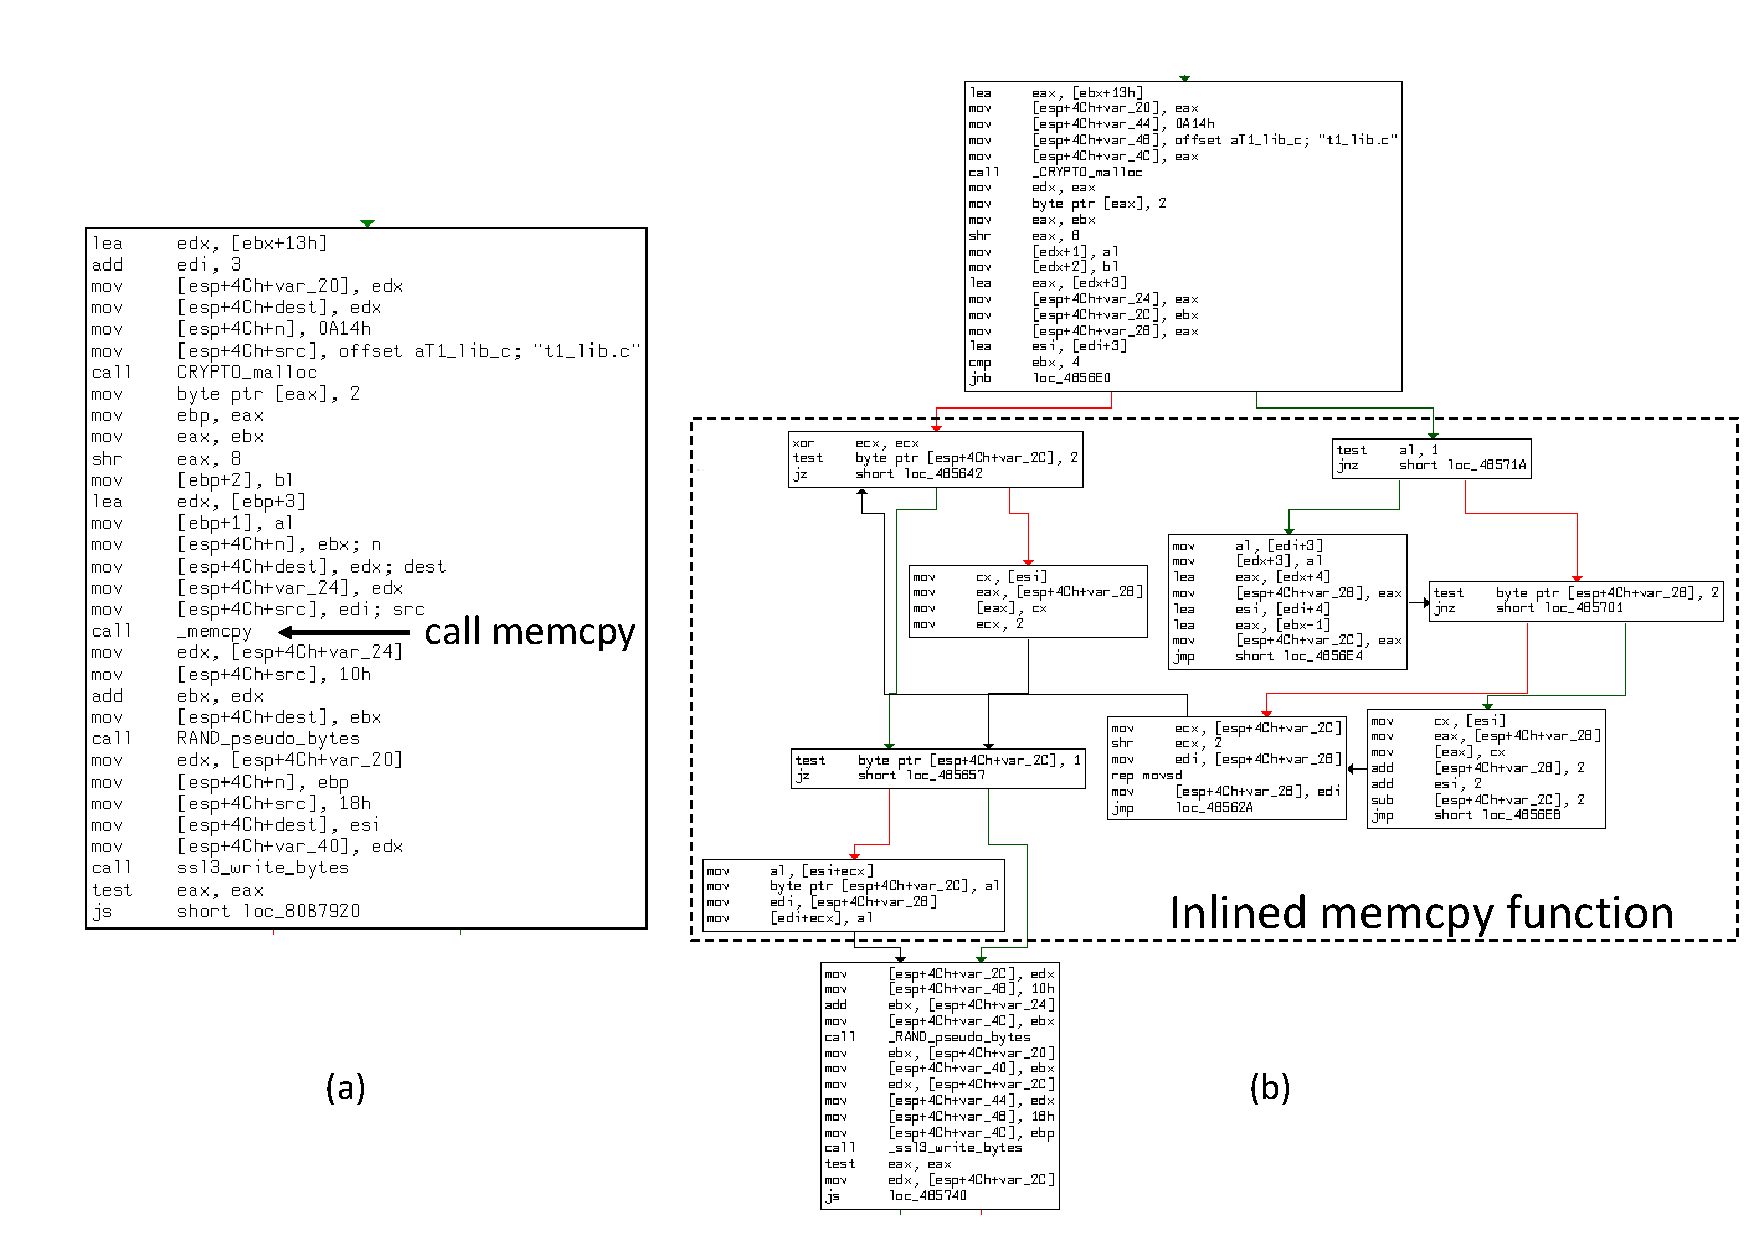
\includegraphics[width=\linewidth]{srj-figures/srj-moti_ex2.pdf}
  \caption{Code segment responsible for Heartbleed vulnerability (CVE-2014-0160) appeared as in the binary (a) compiled with \texttt{gcc} 4.6, and (b) compiled with \texttt{mingw}32} \label{fig:prob_stat}
% \vspace{-4mm}
\end{figure}


\begin{figure*}[th]
  \centering
  \subfigure[String copy via calling function \emph{strcpy}]{
    \label{fig:falseposi:a} %% label for first subfigure
    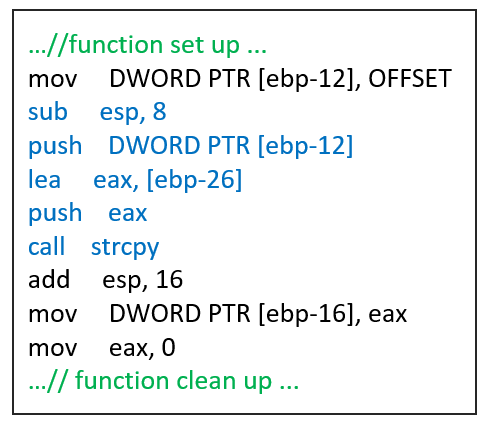
\includegraphics[width=1.8in]{srj-figures/bingoV_exam1a.png}}
  \hspace{1in}
  \subfigure[Memory copy in an iterative way]{
    \label{fig:falseposi:b} %% label for second subfigure
    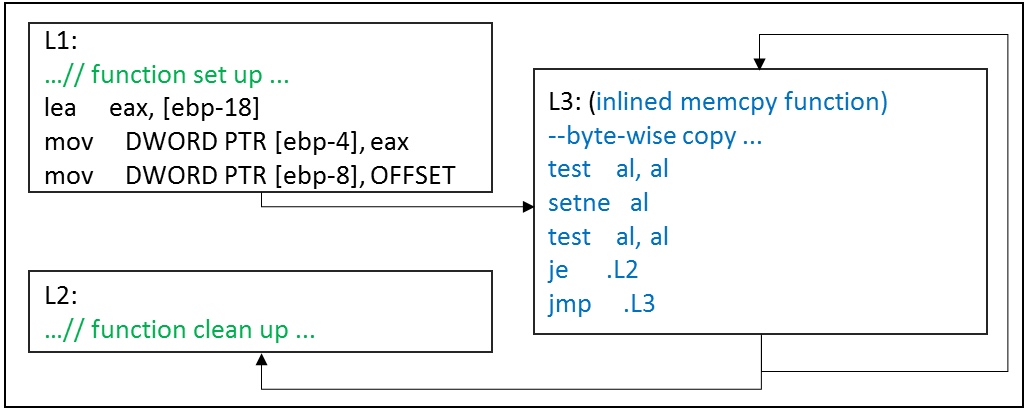
\includegraphics[width=3.82in]{srj-figures/bingoV_exam1b.png}}
  \caption{A false positive case of \tool}
  \label{fig:falseposi} %% label for entire figure
\end{figure*}

\section{Motivation} \label{sec:prob_state}
%Identifying semantically similar or equivalent binary code is a challenging task.
%In this section, %we discuss the problems of the existing binary code search techniques with motivating examples.
%Then
In this section, we state the challenges in the current research of cross-architecture and cross-OS binary code search  with illustrative examples. %We briefly introduce the solutions to these challenges, by leveraging selective inlining, combining different categories of features and adopting emulation.


 %for complete semantics analysis of functions and necessity to have a function model that is agnostic to underlying program structure.
%Then, we introduce the key challenges faced by existing binary function matching tools in detail.

%we \xyx{give a motivating example of binary matching regardless of architecture and OS differences, and state the challenges of  binary code search in finding the semantics and structures for this example. Last, we explain the basic idea of our proposed solution. }%and discuss their roles to achieve the scalable binary matching regardless of architecture and OS differences.}

\subsection{Motivating Example}  \label{subsec:bin_pre}

A binary program consists of a number of functions, each of which can be represented by the CFG (control-flow graph), a (directed) graph of basic blocks (BBs). The assembly instructions in a function are systematically  grouped into several BBs, which are considered as the building blocks of binary program. Thus, this BB-based representation is used by many static binary analysis tools.
%\begin{mydef}
%\emph{(\textbf{Basic-block}) A sequence of assembly instructions without any jumps or jump targets in the middle, where a jump target starts a block, and a jump ends a block.}
%\end{mydef}

%\begin{example}
 The same source code may produce binary code of different BB structures, due to different compilation configurations. Taking the heartbleed vulnerability (CVE-2014-0160) for example, Fig.~\ref{fig:prob_stat}(a) and (b) show the BB structures of the same source code compiled with \texttt{gcc} and \texttt{mingw}, respectively. Apparently, these two binary code segments share no identical BB structures --- with \texttt{gcc}, the vulnerable code is represented as a single basic block;  with \texttt{mingw}, represented as several basic blocks. A detailed inspection suggests that  library function \texttt{memcpy} is inlined in \texttt{mingw} version; while in \texttt{gcc}, it is not. %Due to this library function inlining, in \texttt{mingw}, the similarity between basic-blocks is affected considerably.
%Given the \texttt{gcc} version as a signature, we may miss the vulnerability in \texttt{mingw} version due to the function inlining.
Huge differences between the binaries in syntax and program structure make binary code search a challenging task.
%Hence, basic-block centric
%function modeling similarity matching(\textbf{P1}) and \mahin{program structure dependent pre-fitlering (\textbf{P3})} is not robust enough to address real-world problems. Further, this real-world scenario strongly suggest that functions should not be analysed in isolation, i.e., to capture the true semantics of a functions (\textit{caller}), all the related functions (\textit{callee}) also need to be taken in to consideration based on the caller-callee relationship (\textbf{P2}).
%\end{example}

 % and it is formally defined as follows (adapted from~\cite{david2014tracelet}):
%
%\begin{mydef}
%\emph{(\textbf{Type-k Partial Trace\footnote{In the rest of the sections, we'll use the term `partial trace' and `type-k partial trace' interchangeably, where `type-k partial trace' is used when referring to the length of a partial trace and in all other instances the term `partial trace` is used}}) Type-k partial traces is an ordered tuple of $k$ sequences, each representing one of the basic-blocks in a directed acyclic sub-path in the CFG, and containing all of the basic-block's assembly instructions.
%}
%\end{mydef}



%We introduce the term \emph{environment}, where binary is generated and executed, to denote the underlining architecture (e.g., Intel, ARM), the operating systems (OS) (e.g., Windows, Linux), the used compiler, and also the chosen compilation options.
%Different architectures have different instructions (a.k.a. ISA or Instruction Set Architecture) for the machine.
%Obviously, different environments will lead to considerably different binaries.

%\note{\textbf{I think we need make sure environment is used in the rest of the sections}}


%To better find the assembly code clones that perform similarly computational tasks, we formulate the concept of semantic clones.

% which has very important applications in both software security and software engineering. Despite the challenges, in the recent year, there are several good solutions proposed in academia to tackle this problem~\cite{pewnycross,ruttenberg2014identifying,egele2014blanket,luo2014semantics}. %of identifying semantically equivalent functions at binary level.
%However, none of the existing studies fills up the theory blank of \lq{}how a function is modelled\rq. %In the proposed modelling techniques of {\color{red}{using XXX}}~\cite{pewnycross,luo2014semantics}, it is assumed that basic-block structure is preserved across binaries, and thus, functions models should be  basic-block centric. Based on this assumption, semantic features are extracted from the sample functions at basic-block level and compared with the counterparts extracted from target functions in a pairwise way of basic-block comparison.


\subsection{Challenges for Syntactic Approaches}\label{sec:back:challenge}
Syntax is the most direct information usable for code search.
%However, the key challenge for syntax-based matching is:
%\noindent \textbf{C1: There is no consistent binary syntax representation across architectures.}
%Existing approaches mostly have attempted to use instruction patterns~\cite{DBLP:conf/uss/JangWB13,DBLP:conf/raid/KrugelKMRV05,saebjornsen2009detecting,DBLP:conf/pldi/DavidY14}, where for similarity matching, these approaches rely on syntax information. Though these techniques work well for the given environment (e.g., cases presented in~\cite{DBLP:conf/pldi/DavidY14}), it  fails for cross-architecture analysis, where syntax dramatically changes for different architectures~\cite{DBLP:conf/sp/PewnyGGRH15}.
%%For example, the two binary code segments in Fig. \ref{fig:idiom2-ex}, for ARM (left) and x86 32bit (right) architectures,  both represent the stack frame set up operation in function prologue.
%Hence, it is hard to perform similarity matching across architectures by purely relying on the syntax representation.
Most of existing approaches that rely on syntax information have attempted to use instruction patterns~\cite{DBLP:conf/uss/JangWB13,DBLP:conf/raid/KrugelKMRV05,saebjornsen2009detecting,DBLP:conf/pldi/DavidY14}.
As no consistent low-level syntax representation (i.e., assembly instructions) is available for cross-architecture search, these approaches fail for cross-architecture analysis. %\cite{DBLP:conf/sp/PewnyGGRH15} and CoP~\cite{luo2014semantics} use semantic features (e.g., symbolic expressions) and bug signatures to do cross-architecture analysis, respectively.}
To make binary code search across the architecture and OS boundary, semantics-based matching has been proposed~\cite{luo2014semantics,DBLP:conf/sp/PewnyGGRH15}, in which the machine state transition represents the semantics of a binary. Still, three challenges are faced in semantics-based matching.
%For example, the two binary code segments in Fig. \ref{fig:idiom2-ex}, for ARM (left) and x86 32bit (right) architectures,  both represent the stack frame set up operation in function prologue.

%\begin{figure}[ht]
%\small
% \centering
%  \begin{subfigure}[b]{0.5\linewidth}
%   % \includegraphics[width=0.75\linewidth]{srj-figures/srj-hierarchy-2.png}
%    \raggedright{\texttt{
%    \\
%    	mov ip, sp\\
%    	stm sp!, {fp,ip,lr,pc}\\
%    	sub fp, ip, 16\\
%    }}
%  %  \caption{\small{ARM version}}
%   \label{fig:idiom2-ex-a}
%    \vspace{1ex}
%  \end{subfigure}%%
%   \begin{subfigure}[b]{0.5\linewidth}
%   \centering
%   % \includegraphics[width=0.75\linewidth]{srj-figures/srj-hierarchy-2.png}
%    \raggedright{\texttt{
%    \\
%    	push ebp\\
%    	mov ebp,esp\\
%    	sub esp,16\\
%    }}
% %   \caption{\small{x86 32bit version}}
%   \label{fig:idiom2-ex-b}
%    \vspace{1ex}
%  \end{subfigure}%%
%  \caption{Function prologue for ARM (left) and x86 32bit (right)}
%  \label{fig:idiom2-ex}
%\end{figure}

\subsection{Challenges for Semantics-based Matching} \label{subsec:sem_chall}



\noindent\textbf{C1: The trade-off challenge of deciding the granularity of function model.} %: breaking the limits of basic-block structure.}
The state-of-the-art tools~\textsc{CoP}~\cite{luo2014semantics} and bug search \cite{DBLP:conf/sp/PewnyGGRH15} assume that BB-structure is preserved across binaries, and \xyx{a single BB can be matched with other BBs of similar semantics}. Based on BB-structure, semantic features are extracted and built into the function model. However, as admitted by Pewny \emph{et al.}~\cite{DBLP:conf/sp/PewnyGGRH15}, this approach is too sensitive to BB-structure differences, and hence problematic for smaller functions whose CFG structures are more susceptible to compilation options.
%Based on this, semantic features extracted from the signature function at basic-block level are compared with the counterparts extracted from target functions in a pairwise way.
%\emph{"Our metric is sensitive to the CFG and the segmentation of the basic block, which we found to be potentially problematic especially for smaller functions."}
%In practise, the assumption is too restrictive to be applied for real-world cases.
For example, the BB-structure compiled with  \texttt{gcc} 4.6 in  Fig.~\ref{fig:prob_stat}(a) is significantly different from that compiled with \texttt{mingw}32 in Fig.~\ref{fig:prob_stat}(b). In this case, the approach of BB-centric matching fails as no two BBs can match in Fig.~\ref{fig:prob_stat}.        % semantic features extracted from a single BB in these two cases will not contain the same semantics.





\noindent\textbf{C2. The accuracy challenge of using low-level semantic features.} %: covering the high-level and complete function semantics.}
Functions are considered in isolation by most of static tools, i.e., semantics of callee functions are not considered as part of the caller's semantics. This leads to partial semantics problem, especially when some common utility functions are implemented by the developers themselves (e.g., Adobe Reader has its own \texttt{malloc} implementation).
%Some existing techniques~\cite{wang2015binary} has noticed	the problem of basic-block, and propose to
\textit{Blindly inlining}  all the callee functions can be a remedy, as  all the user-defined functions are inlined in~\cite{wang2015binary}. %The blindly inlining strategy would lead to such a problem of code size explosion that the bloated functions are hard to analyze, incurring heavy overhead.
%However, one might assume that inlining all the callee functions at their respective call sites, as in~\cite{wang2015binary}, would solve the partial (or incomplete) semantics problem present in existing binary function matching techniques.
 Nevertheless, this approach fails in practice due to two main reasons: (1) heavy inlining may lead to code size explosion~\cite{chang1992profile},  %where performing similarity matching on bloated functions incur heavy overhead and hence,
and (2) not all the callee functions are semantically relevant to the caller function. %hence, inlining such functions might dilute the core functionality of the caller function, which in return, leads to poor matching results.
Thus, an inlining strategy is needed to decide that: \texttt{memcpy} should be inlined in Fig.~\ref{fig:prob_stat}(a) for matching with the semantically relevant one in Fig.~\ref{fig:prob_stat}(b). On the other side, \xyx{for functions not to be inlined, e.g., \texttt{ss13\_write\_bytes} in Fig.~\ref{fig:prob_stat}(a), features of library call information should not be ignored.}


\noindent\textbf{C3. The performance challenge of using static symbolic analysis or dynamic execution.} %: replacing with by micro execution.}
 Syntax based techniques, in general, are scalable~\cite{DBLP:conf/pldi/DavidY14}. As discussed earlier, they fail on cross-architecture analysis. To address this problem, semantics based approaches are preferred. However, extracting and solving low-level semantic features is a time-consuming job. Previously, we adopted an \emph{efficient} and architecture-, OS- and compiler-\emph{neutral} function filtering mechanism in \cite{bingo}. \xyx{With such mechanism, extracting input/output values of registers and flags of a function via constraint solving still takes 4,469s on average to extract low-level semantic features from 2,611 Linux \texttt{libc} functions --- it takes 1.7s to extract semantic features from a \texttt{libc} function. Hence, this part still has much space for improvement. To scale up code search for large-size binaries in real world, an efficient method is desired.}

\xyx{Previously, \tool has adopted $k$-tracelet for C1, selective inlining for C2, and filtering mechanism for C3 \cite{bingo}. However, \tool still suffers issues of false positive cases (see Fig.~\ref{fig:falseposi} and \S\ref{subsec:sem_chall_sol}) and inefficient feature extraction. In this paper, \toolNew adopts new features and emulation to address these issues (see \S\ref{sec:category}).}

%Therefore, to facilitate scalable semantic matching, an \emph{efficient}, and architecture, OS and compiler \emph{neutral} function filtering step is required.
%However, exiting approaches focus only on the efficiency aspect of the filter. For example, in~\cite{sebastian2016discovre}, only program structural features, such as number of basic blocks, are used as filters to speed up. However, as shown in Fig.~\ref{fig:prob_stat}, such features are not robust enough for cross-architecture, OS and compiler analysis.

%For example, due to the simplicity of the code in Fig.~\ref{fig:prob_stat}(a), there are many semantically irrelevant functions, which have the same number of basic blocks (i.e., one), to be filtered out before semantic matching.

%
%\noindent\textbf{C2: Semantics of binary code is too low level.}
%Due to the lack of explicit program semantics at binary level, machine state transitions of two totally unrelated code segments may look very similar (or identical), if the number of instructions in those binary segments are too small, e.g., the two code segments in Fig.~\ref{fig:code_seg}.
%A binary modeling approach based on machine state transitions has the problem of producing high false positives, especially when the given function (or vulnerability) signature is too small~\cite{DBLP:conf/sp/PewnyGGRH15}.
%%\ly{combine fig 2 and 3?}
%%Unfortunately, signatures, especially vulnerability signatures, having few instructions is common in real-world scenarios~
%
%\begin{figure}[t]
% \begin{center}
% \subfigure[A code segment to XX]{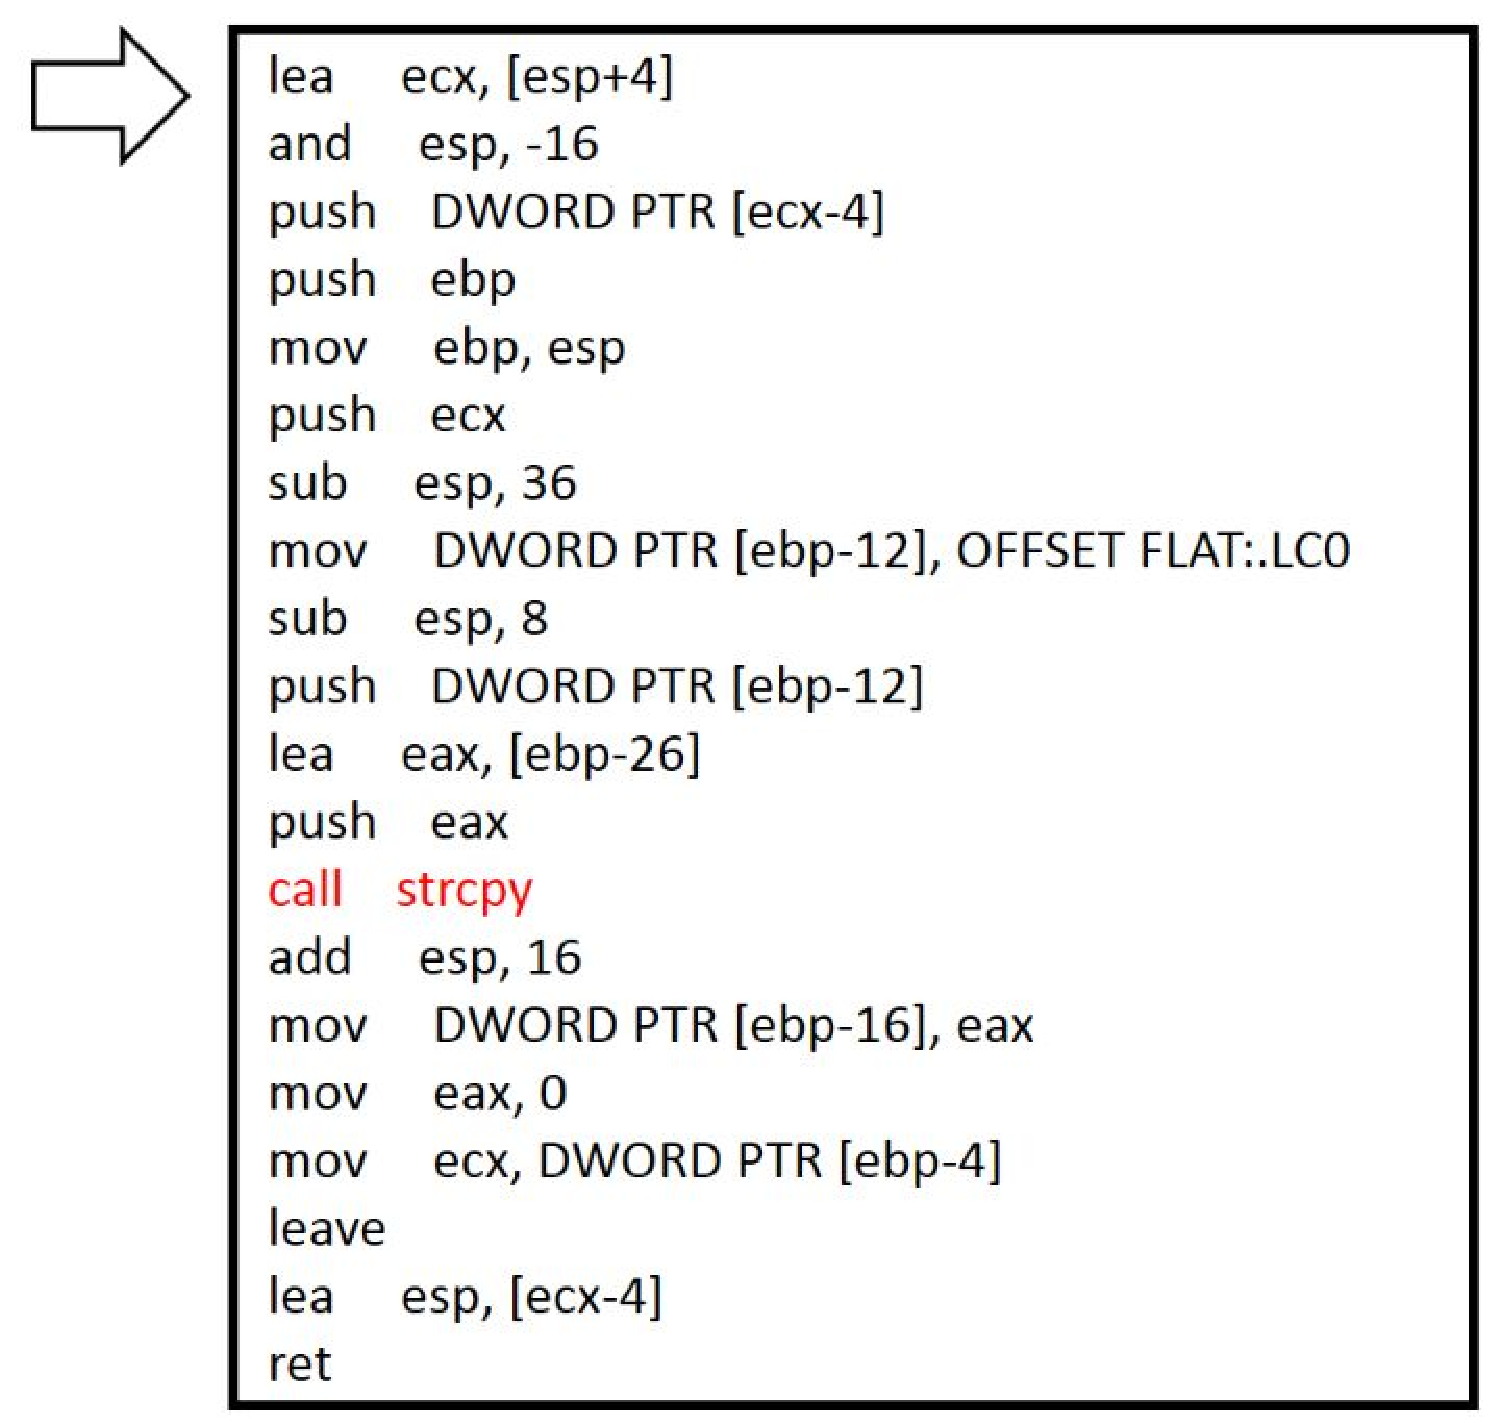
\includegraphics[width=200pt]{srj-figures/runexample1.pdf}}\label{fig:seg1:a}
% \subfigure[A code segment to XX]{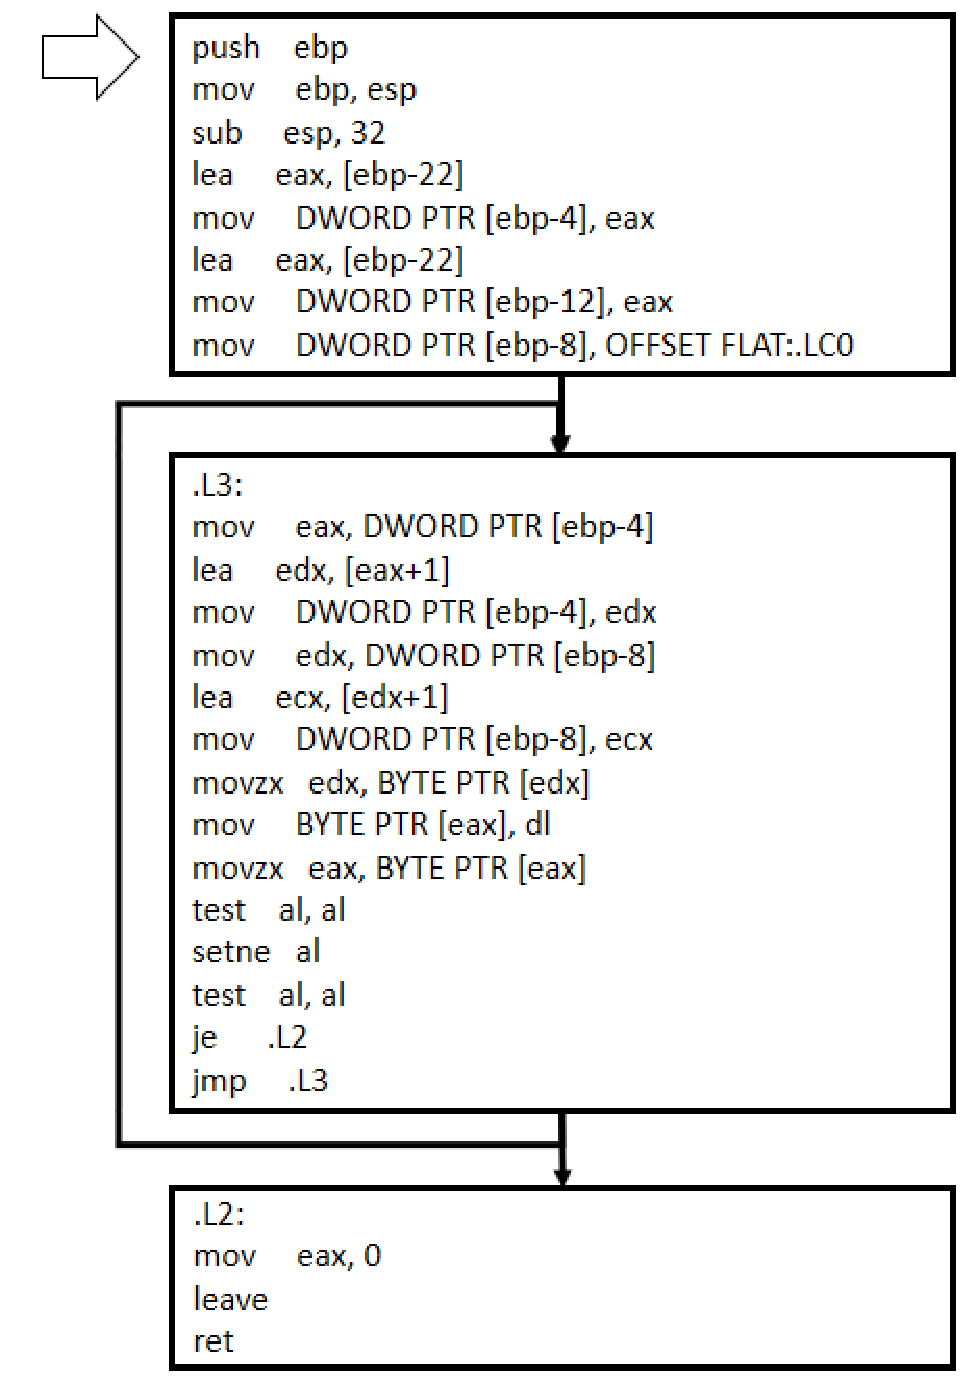
\includegraphics[width=200pt]{srj-figures/runexample2.pdf}}\label{fig:seg1:b}
%\end{center}
%\vspace{-4mm}
%\caption{\toolNew system architecture}
%\label{fig:code_seg}
%
%\end{figure}

%
%As shown in Fig. \ref{fig:state_seg}, two unrelated segments in Fig.~\ref{fig:code_seg} have the same initial machine state (i.e., pre-state) and also the identical post-state after execution. %, both code segments will result in .
%Here, code segment 1 adds the values in $\mathtt{EAX}$ and $\mathtt{EBX}$ registers, and move the results to $\mathtt{EAX}$ register. Since the pre-state values are all set to zero, after execution, $\mathtt{EAX}$ register will hold the value 0 and the condition-code flag $\mathtt{ZF}$ (zero flag) will be set to 1, since the result of addition operation is zero. On the other hand, in code segment 2, the value in $\mathtt{EBX}$ register is pushed to the stack, system API $\mathtt{strlen}$ is invoked, and finally the return value that is stored in $\mathtt{EAX}$ register is compared with an immediate value `0'. After execution, similar to code segment 1, $\mathtt{EAX}$ register will hold the value 1 as $\mathtt{strlen}$ system API is not interpreted (e.g., \cite{DBLP:conf/sp/PewnyGGRH15,luo2014semantics}), $\mathtt{EAX}$ register will hold the pre-state value, which is 0. In addition, the comparison operation will set the $\mathtt{ZF}$ to 1. In both executions, none of the other registers, condition-code flags and memory locations will be modified, hence retaining the pre-state values. From the examples shown in Fig.~\ref{fig:code_seg} and~\ref{fig:state_seg}, it can be seen that machine state transitions alone are not sufficient to model binary code.
%%\end{example}

%\noindent \textbf{C3: Computing the precise semantics is difficult and expensive.}
%Static methods~\cite{luo2014semantics,DBLP:conf/sp/PewnyGGRH15} using state-based semantic computation cannot capture the precise semantics due to missing the consideration of system APIs in the analysis.
%Dynamic analysis based techniques such as~\cite{egele2014blanket} might be able to address this problem. However, it is not scalable enough to handle large binaries. For example, in \cite{egele2014blanket}, before each function is executed, an environment needs to be set so that the execution does not terminate due to uninitialised memory handling. Unfortunately, considering the fact that a moderate size binary would easily have several thousand functions, this approach is not very scalable. %Hence, to address these challenges, we propose a partial traces based function modelling technique.







%\begin{mydef} \label{def:tracelet}
%\emph{\textbf{A partial trace} is \note{an instruction sequence obtained from basic-blocks that lie adjacent to each other along a program execution path. Partial traces can be of different length, where partial trace of length $k$ (called, Length-$k$ partial trace) denotes a partial trace that contains the instructions obtained from $k$ adjacent basic-blocks that lie along a program execution pat }}
%\end{mydef}
%
%\begin{mydef} \label{def:comp_semantic}
%\emph{\xyx{\textbf{Complete (or true) Semantics} refer to the contextual semantics that the function under analysis and %why we need true semantics of a function because compiler inline/outline certain functions
%}}
%\end{mydef}


%As discussed in Section \ref{sec:prob_state},
%The existing static binary function matching techniques, in general, fail to take into account the true (or complete) semantics of the functions under investigation. That is, each function in a binary is analyzed in isolation, where the semantics of the callee functions (be it user-defined or library function) are not considered when generating the caller function semantics as they are assumed to be two different functions. However, this assumption is intuitive and valid until we understand the caller-callee relationship (or dependency). For example, assume a user-defined function that manipulates string literals invokes the \texttt{strcpy} library function, and in order to capture the true semantics of the caller, it is \note{essential?} to inline \texttt{strcpy} function at the call site, as the caller function is involved in string manipulation, where it leverages on utility fucntions, such as \texttt{strcpy}, provided by the C runtime library to simplyfy its operations, hence, the semantics of the utility functions need to be considered as part of the caller fucntion semantics. Similarly, in another occasion, the programmer might implement her own version of \texttt{strcpy} function with additional security properties (called, \texttt{strcpy\_secure}\footnote{It is worth noting that \texttt{strcpy} is one of the banned function calls by Microsoft and hence, its better to use more secure variants such as \texttt{strncpy\_s} and \texttt{strcpy\_s}~\cite{msbannedfunctioncalls}}) and invokes it from all the string manipulation functions that need a secure string copy operation, hence, to capture the true caller semantics, the user-defined \texttt{strcpy\_secure} function needs to be inlined at the call site.

%To this end, in this paper, we propose partial trace based function modelling to overcome the aforementioned limitation.

%\noindent\textbf{$3$-tracelet or $k$-tracelet?}  In \cite{DBLP:conf/pldi/DavidY14}, $3$-tracelet, a concatenation of 3 adjacent basic-blocks, is used for searching. \textcolor{red}{Why k-tracelet is better.}


%Semantic based vulnerability detection at binary code level is an active research area and a promising direction towards securing closed-source software programs. However, we find that there is a gap in existing work \cite{pewnycross}\cite{ruttenberg2014identifying}, especially in vulnerability modelling, that is worth exploring. In the proposed vulnerability modelling techniques, it is assumed that basic-block structure is preserved across binaries \cite{pewnycross}, and thus, vulnerabilities are modelled basic-block centric. That is, semantic features are extract for from the basic-blocks in the known vulnerable function and they are compared with the basic-blocks in the target functions to identify the staring points of potential vulnerabilities.

%In \cite{ruttenberg2014identifying}, it is reported that for each basic-block in the signature (called, \textit{starting points}), first 20 basic-blocks (in-terms of similarity), in the target program, are selected for further signature matching. Similarly, in \cite{pewnycross}, for each basic-block in the signature, first 200 candidate basic-blocks, in the target program, are selected for the next level of vulnerability signature matching, using a greedy BHB (Best-Hit Boarding) algorithm. The commonality between these approaches is that the starting points, for vulnerability signature matching, are selected based on the similarity between basic-blocks in signature and target programs. However, the major drawback in this approach is that the basic-block structures can be easily distorted by factors that are beyond the control of security analysts.

%For example, figure \ref{fig:prob_stat}(a) shows the well-known heartbleed vulnerability (CVE-2014-0160) that shook the entire software industry. Figure \ref{fig:prob_stat}(a) shows the vulnerability at binary code level, compiled with GCC-4.6 and (c) shows the same vulnerability, but compiled with MinGW32. Immediately, we can say that the two programs doesn't share same basic-block structure. That is, with GCC, the vulnerable code is represented as a single basic-block, however, with MinGW, it is split into several basic-blocks. A deeper inspection would suggest that in MinGW version the library function \texttt{memcpy} is inlined while in GCC, it is not. Due to this library function inlining, in MinGW, the similarity between basic-blocks is affected considerably. That is, given the GCC version as a signature, we may miss the vulnerability in MinGW version due to basic-block \textit{splitting} and \textit{vice-versa} due to basic-block \textit{merging}. Hence, basic-block centric vulnerably modelling may not be robust against factors such as compiler type (version), optimization level and even difference in build environments. Therefore, in this paper, we present a more robust, self-adoptable vulnerability modelling technique.

%\todo {\color{blue} Do I need to include scope here? like doesn't not consider obfuscated binary that are hard to disassemble and only consider clean binaries without any obfuscations/packing.}

%\subsection{Problem Statement and Possible Solution} \label{subsec:pos_sol}
%To compare binaries, we need to define the criteria to compute similarity.
%In this work, we propose two complementary criteria to capture the semantic and structural information of the binary programs.
%Let $\mathcal{I}_1$ and $\mathcal{I}_2$ be two partial traces, we formally define the two kinds of similarity as follows:
%%The function $\langle\!\langle inst \rangle\!\rangle$ converts an instruction sequence (or an instruction) into a corresponding symbolic expression.
%
%
%\begin{mydef} \label{def:sem_sim}
%\emph{(\textbf{Semantic Similarity})
%Let $s_0$ denote a pre-state before executing $\mathcal{I}$, and $s_1=\langle\!\langle s_0, \mathcal{I}\rangle\!\rangle$ denote post-state after executing $\mathcal{I}$ on $s_0$. %post_\mathcal{I}^{pre_{\mathcal{I}}}=
%Let $S$ be set of all possible pre-states values that both $\mathcal{I}_1$ and $\mathcal{I}_2$ can execute on.
%The semantic similarity of $\mathcal{I}_1$ and $\mathcal{I}_2$, $SemSim(\mathcal{I}_1, \mathcal{I}_2)$, is defined as
%$\sum\nolimits_{s \in S} (\langle\!\langle s, \mathcal{I}_1\rangle\!\rangle -_m \langle\!\langle s, \mathcal{I}_2\rangle\!\rangle)$, where $-_m$ is a function to measure the difference of two machine states.
%%, the function $\langle\!\langle \bullet \rangle\!\rangle$ converts a partial trace into a set of \emph{symbolic expressions} and $\langle\!\langle \mathcal{I} \rangle\!\rangle(s)$ denotes assigning pre-state values $s$ to the symbolic expressions to yield the post-state values $ \mathcal{I}(s)$
%% are so \emph{similar in IO semantics} that they perform the similar computation tasks, if $PreS(\mathcal{I}_1)\approx reS(\mathcal{I}_2)$ and $PostS(\mathcal{I}_1)\approx PostS(\mathcal{I}_2)$.
%}
%\end{mydef}
%
%
%%In this work, a machine state is defined by the values stored at registers, condition-code flags and memory locations, which are common in all computing architectures.
%Semantic similarity is defined to capture the difference of the effects (i.e., post-state) of the binary program execution from the same input.
%Note that to calculate the precise effects of the program, we also need to consider the OS relevant information, like system API.
%Therefore, we consider that semantic similarity is architecture independent and OS dependent.
%
%%\ly{give one example of two code seg with different syntax, but same semantics}
%%Like example two in Fig. \ref{fig:state_seg}, the two code segments are not necessary to be from the same architecture, as the state model is not based on information that is architecture specific (see Section XX).
%
%Semantic similarity is one essential criteria to capture the behavior similarity of programs.
%However, this definition ignores the difference of program's structures, i.e., the program is treated as a black box.
%Due to the challenge \textbf{C2}, when comparing two binaries, we also want to consider the structures of the binary to make sure they are implementing the same algorithm or computation.
%%For example, bubble sort should not match with quick sort although they are semantically identical.
%This is critical in the tasks like code auditing, plagiarism detection and vulnerability detection.
%
%\begin{mydef} \label{def:comp_sim}
%\emph{(\textbf{Structural Similarity})
%The structural similarity of $\mathcal{I}_1$ and $\mathcal{I}_2$, $StrSim(\mathcal{I}_1, \mathcal{I}_2)$, is defined as
%$f^p_a(\mathcal{I}_1) -_f f^{p'}_{a'}(\mathcal{I}_2)$, where  $f^{p}_a(\mathcal{I}_1)$ (or $f^{p'}_{a'}(\mathcal{I}_2)$) is an abstraction function that maps $\mathcal{I}_1$ (or $\mathcal{I}_2$) to a structural model on architecture $a$, OS $p$ (or on architecture $a'$, OS $p'$); and $-_s$ is a function to measure the difference of two structural models.
%}
%\end{mydef}
%
%
%Structural similarity is a general definition. %, which aims to capture the high-level behavior of the binary code.
%The actual design of the abstraction function $f$ (e.g., using instruction patterns: $n$-gram~\cite{DBLP:conf/uss/JangWB13}, graphlet~\cite{DBLP:conf/raid/KrugelKMRV05} and tracelet~\cite{DBLP:conf/pldi/DavidY14}) reflects different research approaches on how to abstract the structural information of the binaries.
%Other usable structural information includes AST, PDG, data flow, type information and loop information.
%%For example, AST and PDG have been widely used for clone detection which reflect the syntax similarity.
%It is clear that the abstraction function is usually architecture and OS dependent, e.g., the codes in Fig.~\ref{fig:idiom2-ex}.
%%(e.g., using AST, PDG, data flow, type information, API and loop information)
%%Since the structureal information of assembly code (e.g., CFG) is usually architecture and OS specific, the direct matching based on CFG is not accurate, as shown in Fig. \ref{fig:prob_stat}. In this paper, we consider program information beyond the syntactic structure of the assembly code --- in addition, we also consider  data flow, type, API and loop information.
%
%%To capture the information relevant to semantics, we mainly consider data flow, API and partial traces in our model, while the structural information like BB is not the focus of our model.
%
%
%Overall, the similarity of $\mathcal{I}_1$ and $\mathcal{I}_2$ is defined as the combination of their semantic similarity and structural similarity.
%This similarity definition naturally resolves the challenge \textbf{C2}.
%
%To solve \textbf{C1}, we need to define a structural model, which is robust to different architectures and OSs. Motivated by the recent work on source code level idiom mining~\cite{allamanis2014mining},
%we propose to use the common binary patterns in different architectures and OSs as idioms, and use idioms to capture the program structural information, i.e., to define the abstraction function $f$.
%To support cross environments analysis, we propose a mapping of idioms in different architectures and OSs to a common concept such that $-_s$ can be easily computed.
%
%To solve \textbf{C3}, we propose a static analysis to capture the state-based semantics~\cite{DBLP:conf/sp/PewnyGGRH15} so that our approach is scalable.
%To capture the missing semantics related to system API using the static analysis, we introduce API idioms to complete the semantic information.
%Although the semantic comparison in this way is not precise as dynamic analysis like~\cite{egele2014blanket}, it works well with good scalability as shown in experiments.
%Furthermore, the idiom approach addresses the OS dependency problem in the semantic similarity definition.
%
%To solve \textbf{C4}, we propose a partial trace based function modeling, where partial traces of various lengths are extracted from binary code segment and they are organized in a systematic manner to handle program structure distortion. That is, by using partial trace models, no assumptions about the signature and target program structures are made (as in Tracy~\cite{DBLP:conf/pldi/DavidY14}).
%%However, in \tool, partial traces of varying lengths are considered, which doesn't make any assumption about the program structure}
%%By combining static analysis and feature hashing~\cite{jang2011bitshred}, our approach is scalable as no dynamic analysis is required.
%Overall, the unified idiom models for different environments make our solution work for all architectures and OSs.  The partial trace function modeling and complete semantic information give an accurate solution.
%
%
%%Different from \cite{allamanis2014mining}, the idiom mining is based on the tracelet from binary code and date dependency analysis. Our model is to capture the high level semantics of the assembly code, such as the idioms that abstract away the low level details, by which we search for the semantically similar assembly code regardless of architecture or OS differences,
%
%
%
%%In binary code similarity matching, due to the compilation process and optimizations, the syntax information is largely different.
%%
%% A desired model is needed to detect the assembly code in Fig \ref{fig:prob_stat} as similar, but the example in Fig \ref{fig:code_seg} not as similar. Hence, the model should be resistent to the syntactic differences due to BB structures, meanwhile, not encumbered by the issues of the pure similarly analysis of semantics. Hence, to strike a balance, we propose a partial trace (tracelet) based assembly code modeling technique.
%
%
%%To sum up, the computation model should leverages the static analysis for gaining the information from the three aspects: IO semantic based  model at the low level, tracelet based model at the middle level and idiom \cite{allamanis2014mining} based model at the high level.
%
